\documentclass[12pt]{article}
\usepackage[utf8]{inputenc}
\usepackage[T1]{fontenc}
%\usepackage{fullpage}
%\usepackage{psfig}
\usepackage{times}
\usepackage{xspace}
\usepackage[hyphens]{url}
\usepackage{geometry}
\usepackage{graphicx}
%\usepackage[tight]{subfigure}
\usepackage{array}
\usepackage{makecell}
\usepackage{multicol}
\usepackage{algorithm}
\usepackage{algorithmic}
\usepackage{amssymb}
\usepackage{amsmath}
\usepackage{amsfonts}
\usepackage{fancyhdr}
\usepackage{booktabs}
\usepackage{listings}
\usepackage{ifthen}
\usepackage{wrapfig}
\usepackage[sort,compress,numbers]{natbib}
\usepackage[compact]{titlesec}
\usepackage[usenames,dvipsnames]{xcolor}
%\usepackage{comment}

% \usepackage[hidelinks]{hyperref}
\usepackage{multirow}
\usepackage{framed}
\usepackage{enumitem}
\usepackage[font=footnotesize,font=bf,it]{caption} 
\usepackage{epstopdf} 
%\usepackage{subfig, enumerate}
\usepackage{subcaption}
\usepackage{csquotes}
\usepackage{tabularx}
\usepackage{beramono}
\usepackage{pdfpages}
\PassOptionsToPackage{hyphens}{url}\usepackage[colorlinks=true,urlcolor=blue]{hyperref}

\urlstyle{same}
\usepackage{wrapfig}

\definecolor{dkgreen}{rgb}{0,0.6,0}
\definecolor{gray}{rgb}{0.5,0.5,0.5}
\definecolor{mauve}{rgb}{0.58,0,0.82}

\newcommand{\proptitle}{Sandia Technical Report: Balar: SST/GPGPU-Sim Integration}
\newcommand{\shorttitle}{Balar}

\newcommand{\system}{\shorttitle\xspace}

\geometry{verbose,papersize={8.5in,11in},
		left={1in},right={1in},top={1in},bottom={1in}}
\pagestyle{fancy}
\lhead{Purdue University: \shorttitle}
\rhead{Sandia TR}
\renewcommand{\footrulewidth}{0.4pt}
\lfoot{Purdue University, Sandia National Labs}
\cfoot{}
\rfoot{\thepage}



% \def\IncSpacing{\addtolength{\baselineskip}{0.5\baselineskip}}
% \def\IncSpacing{\addtolength{\baselineskip}{0.22\baselineskip}}
% \def\DecSpacing{\addtolength{\baselineskip}{-0.33333\baselineskip}}

%\newfont{\cour}{cmtt10}

%\renewcommand{\paragraph}[1]{\medskip\noindent\textbf{#1.}}
% \renewcommand{\paragraph}[1]{\smallskip\noindent\textbf{#1.}}

% \setlength{\itemsep}{20pt}
\addtolength{\itemsep}{-1in}
% Reduce spacing in lists
\setlist[itemize]{noitemsep} % noitemsep -> nosep will make it even more compact, but not advisable
\setlist[enumerate]{noitemsep}
\setlist[description]{noitemsep}
% \setlist{notopsep}
% \setlist{parskip=0pt}
% \setlist[enumerate]{listparindent=3ex}
% \setlist[enumerate]{itemindent=1ex}
% \setlist{leftmargin=0pt}

 \iftrue % Change this to \iffalse to hide all the comments.
%\iffalse
\newcommand{\grumbler}[3]{\color{#3}{\sl{\bf #1:} #2}\color{black}}
\else
\newcommand{\grumbler}[3]{}
\fi

\newcommand{\milind}[1]{\grumbler{MK}{#1}{blue}}
\newcommand{\bjm}[1]{\grumbler{BM}{#1}{purple}}
% \newcommand{\propdets}[1]{\grumbler{From call}{#1}{orange}}
\newcommand{\propdets}[1]{}
\newcommand{\fixme}[1]{\grumbler{Fixme}{#1}{red}}


\newcommand{\ie}{{i.e.,}\xspace}
\newcommand{\eg}{{e.g.,}\xspace}
\newcommand{\etal}{{et al.}\xspace}

\newcommand\invisiblesubsection[1]{%
  \refstepcounter{subsection}%
  \addcontentsline{toc}{subsection}{\protect\numberline{\thesubsection}#1}%
  \sectionmark{#1}}

%\renewcommand{\baselinestretch}{0.975}

\renewcommand{\thesection}{\Alph{section}}

\begin{document}

\pagenumbering{roman}

\title{\proptitle}


\newpage

\pagenumbering{arabic}

Programmable accelerators have become commonplace in modern computing systems.
Advances in programming models and the availability of massive amounts of data
have created a space for massively parallel acceleration where the context for
thousands of concurrent threads are resident on-chip. These threads are grouped
and interleaved on a cycle-by-cycle basis among several massively parallel
computing cores. The design of future supercomputers relies on an ability to
model the performance of these massively parallel cores at scale.

To address the need for a scalable, decentralized GPU model that can model large
GPUs, chiplet-based GPUs and multi-node GPUs, this report details the first
steps in integrating the open-source, execution driven GPGPU-Sim into the SST
framework. The first stage of this project, creates two elements: a kernel
scheduler SST element accepts work from SST CPU models and schedules it to an
SM-collection element that performs cycle-by-cycle timing using SST’s
MemHierarchy to model a flexible memory system.
%Initial results indicate a close
%correlation between the new GPU-SST model and real hardware.

With the rise of General-Purpose Graphics Processing Unit (GPGPU) computing and
compute-heavy workloads like machine-learning, compute accelerators have become
a necessary component in both high-performance supercomputers and
datacenter-scale systems. The first exascale machines are expected to heavily
leverage the massively parallel compute capabilities of GPUs or other highly
parallel accelerators \cite{snl_roadmap}. As the software stack and programming model of GPUs and
their accelerator peers continue to improve, there is every indication that
this trend will continue. As a result, architects that wish to study the design
of large-scale systems will need to evaluate the effect that their techniques have
using a GPU model. However, the focus of all publicly available cycle-level
simulators ({\em e.g}GPGPU-Sim \cite{gpgpu_sim}) to date, has been on single-node
simulation performance. In order to truly study
the problem at scale, or for the simulation of large workloads, a parallelizable,
multi-node GPU simulator is necessary.

   \begin{figure}[!htb]
      \centering
      \setlength{\abovecaptionskip}{6pt plus 1pt minus 1pt}
      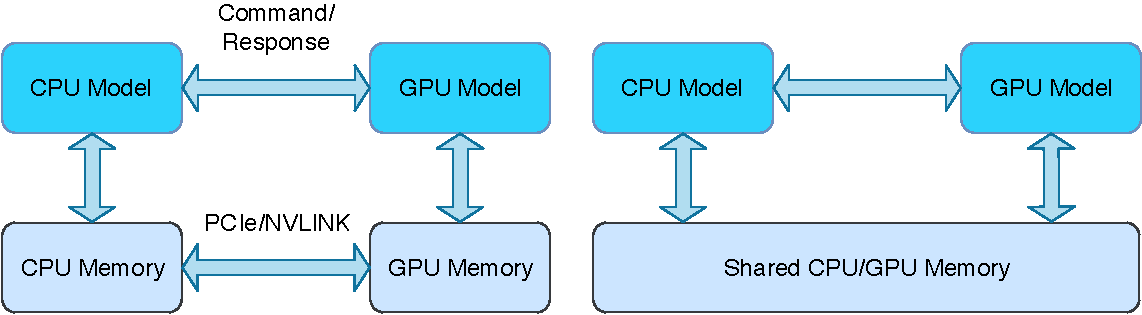
\includegraphics[width=.85\textwidth,keepaspectratio]{figures/cpu_gpu_model.pdf}
      \captionsetup{width=.75\textwidth}
      \caption{High-level CPU/GPU interaction model}
      \label{fig:model}
   \end{figure}

Figure~\ref{fig:model} depicts the current CPU/GPU model co-processor model.
On the left is the common high-performance, discrete GPU configuration, where the CPU
and GPU have separate memory spaces and are connected via either PCIe or a
high-bandwidth link (such as NVLink). The right shows an Accelerated Processing Unit (APU
 model where the CPU
and GPU share a single memory. Note that in even in the discrete memory case, modern
memory translation units allow the CPU and GPU to share the same virtual address space,
although the memories themselves are discrete components.

In this report we will detail a model that is capable of simulating both
discrete and unified memory spaces by leveraging the MemHeirarchy interface in
SST \cite{sst}. This report details our efforts to integrate the functional and streaming
multiprocessor core models from the open-source simulator GPGPU-Sim into SST.

The first step in integrating GPGPU-Sim into SST is to handle the interaction
with an SST CPU component. Since GPUs today function solely as co-processors,
functionally executing GPU-enabled binaries requires the CPU to initialize and
launch kernels of work to the GPU. In our model, the GPU is constructed out of
two discrete SST components -- a scheduler and a SM block \cite{v100}. When CUDA
functions are called from the CPU component, they are intercepted and translated
into messages that are sent over SST links to the GPU (along with the associated
parameters). Table \ref{tab:apis} enumerates the CUDA API calls currently intercepted
and sent to the GPU elements. These calls are enough to enable the execution of
a number of CUDA SDK kernels, DoE proxy apps as well as a collection of Kokkos Unit
tests. Table \ref{tab:kokkos_tests} lists the number of Kokkos unit tests that
pass with our current implementation of SST-GPU, which is about 60\%. There is
ongoing work with the PTX parser to increase the number of running kernels.


    \begin{table}[!htbp]
        \centering
        \setlength{\abovecaptionskip}{6pt plus 1pt minus 1pt}
        \captionsetup{width=.75\textwidth}
        \caption {Intercepted CUDA API Calls Forwarded to GPU Model}
            \begin{tabular}{|p{14cm} | p{3cm}|}
%             \multicolumn{1}{c} {\textbf{API Call}} \\
            \hline
            \texttt{\textunderscore \textunderscore cudaRegisterFatBinary} \\
            \hline
            \texttt{\textunderscore \textunderscore cudaRegisterFunction} \\
            \hline
            \texttt{cudaMalloc} \\
            \hline
            \texttt{cudaMemcpy} \\
            \hline
            \texttt{cudaConfigureCall} \\
            \hline
            \texttt{cudaSetupArgument} \\
            \hline
            \texttt{cudaFree} \\
            \hline
            \texttt{cudaLaunch} \\
            \hline
            \texttt{cudaGetLastError} \\
            \hline
            \texttt{\textunderscore \textunderscore cudaRegisterVar} \\
            \hline
            \texttt{cudaOccupancyMaxActiveBlocksPerMultiprocessorWithFlags} \\
            \hline
            \end{tabular}
        \label{tab:apis}
    \end{table}

      \begin{table}[!htbp]
         \centering
         \setlength{\abovecaptionskip}{6pt plus 1pt minus 1pt}
         \captionsetup{width=.75\textwidth}
         \caption {Functionally Passing Kokkos Unit Tests}
            \scalebox{0.56}{
            \tabcolsep=0.11cm\begin{tabular}{lll}
               \multicolumn{1}{c}{\textbf{Kernel Name}} & \multicolumn{1}{c}{\textbf{GPGPU-Sim}} & \multicolumn{1}{c}{\textbf{GPGPU-Sim/SST}} \\
               abs\_double & {\color[HTML]{32CB00} OK} & {\color[HTML]{32CB00} OK} \\
               abs\_mv\_double & {\color[HTML]{32CB00} OK} & {\color[HTML]{32CB00} OK} \\
               asum\_double & {\color[HTML]{32CB00} OK} & {\color[HTML]{32CB00} OK} \\
               axpby\_double & {\color[HTML]{32CB00} OK} & {\color[HTML]{32CB00} OK} \\
               axpby\_mv\_double & {\color[HTML]{32CB00} OK} & {\color[HTML]{32CB00} OK} \\
               axpy\_double & {\color[HTML]{32CB00} OK} & {\color[HTML]{32CB00} OK} \\
               axpy\_mv\_double & {\color[HTML]{32CB00} OK} & {\color[HTML]{32CB00} OK} \\
               dot\_double & {\color[HTML]{32CB00} OK} & {\color[HTML]{32CB00} OK} \\
               dot\_mv\_double & {\color[HTML]{32CB00} OK} & {\color[HTML]{32CB00} OK} \\
               mult\_double & {\color[HTML]{32CB00} OK} & {\color[HTML]{32CB00} OK} \\
               mult\_mv\_double & {\color[HTML]{32CB00} OK} & {\color[HTML]{32CB00} OK} \\
               nrm1\_double & {\color[HTML]{32CB00} OK} & {\color[HTML]{32CB00} OK} \\
               nrm1\_mv\_double & {\color[HTML]{32CB00} OK} & {\color[HTML]{32CB00} OK} \\
               nrm2\_double & {\color[HTML]{32CB00} OK} & {\color[HTML]{32CB00} OK} \\
               nrm2\_mv\_double & {\color[HTML]{32CB00} OK} & {\color[HTML]{32CB00} OK} \\
               nrm2\_squared\_double & {\color[HTML]{32CB00} OK} & {\color[HTML]{32CB00} OK} \\
               nrm2\_squared\_mv\_double & {\color[HTML]{32CB00} OK} & {\color[HTML]{32CB00} OK} \\
               nrminf\_double & {\color[HTML]{FE0000} FAILED} & {\color[HTML]{9B9B9B} PREVIOUS FAILED} \\
               nrminf\_mv\_double & {\color[HTML]{FE0000} FAILED} & {\color[HTML]{9B9B9B} PREVIOUS FAILED} \\
               reciprocal\_double & {\color[HTML]{FE0000} FAILED} & {\color[HTML]{9B9B9B} PREVIOUS FAILED} \\
               reciprocal\_mv\_double & {\color[HTML]{FE0000} FAILED} & {\color[HTML]{9B9B9B} PREVIOUS FAILED} \\
               scal\_double & {\color[HTML]{32CB00} OK} & {\color[HTML]{32CB00} OK} \\
               scal\_mv\_double & {\color[HTML]{32CB00} OK} & {\color[HTML]{32CB00} OK} \\
               sum\_double & {\color[HTML]{32CB00} OK} & {\color[HTML]{32CB00} OK} \\
               sum\_mv\_double & {\color[HTML]{32CB00} OK} & {\color[HTML]{32CB00} OK} \\
               update\_double & {\color[HTML]{32CB00} OK} & {\color[HTML]{32CB00} OK} \\
               update\_mv\_double & {\color[HTML]{32CB00} OK} & {\color[HTML]{32CB00} OK} \\
               gemv\_double & {\color[HTML]{FE0000} FAILED} & {\color[HTML]{9B9B9B} PREVIOUS FAILED} \\
               gemm\_double & {\color[HTML]{FE0000} FAILED} & {\color[HTML]{9B9B9B} PREVIOUS FAILED} \\
               sparse\_spgemm\_double\_int\_int\_TestExecSpace & {\color[HTML]{FE0000} FAILED} & {\color[HTML]{9B9B9B} PREVIOUS FAILED} \\
               sparse\_spadd\_double\_int\_int\_TestExecSpace & {\color[HTML]{FFC702} NOT PARSED} & {\color[HTML]{9B9B9B} PREVIOUS FAILED} \\
               sparse\_gauss\_seidel\_double\_int\_int\_TestExecSpace & {\color[HTML]{FFC702} NOT PARSED} & {\color[HTML]{9B9B9B} PREVIOUS FAILED} \\
               sparse\_block\_gauss\_seidel\_double\_int\_int\_TestExecSpace & {\color[HTML]{FFC702} NOT PARSED} & {\color[HTML]{9B9B9B} PREVIOUS FAILED} \\
               sparse\_crsmatrix\_double\_int\_int\_TestExecSpace & {\color[HTML]{FFC702} NOT PARSED} & {\color[HTML]{9B9B9B} PREVIOUS FAILED} \\
               sparse\_blkcrsmatrix\_double\_int\_int\_TestExecSpace & {\color[HTML]{FFC702} NOT PARSED} & {\color[HTML]{9B9B9B} PREVIOUS FAILED} \\
               sparse\_replaceSumIntoLonger\_double\_int\_int\_TestExecSpace & {\color[HTML]{FFC702} NOT PARSED} & {\color[HTML]{9B9B9B} PREVIOUS FAILED} \\
               sparse\_replaceSumInto\_double\_int\_int\_TestExecSpace & {\color[HTML]{FFC702} NOT PARSED} & {\color[HTML]{9B9B9B} PREVIOUS FAILED} \\
               sparse\_graph\_color\_double\_int\_int\_TestExecSpace & {\color[HTML]{FFC702} NOT PARSED} & {\color[HTML]{9B9B9B} PREVIOUS FAILED} \\
               sparse\_graph\_color\_d2\_double\_int\_int\_TestExecSpace & {\color[HTML]{FE0000} FAILED} & {\color[HTML]{9B9B9B} PREVIOUS FAILED} \\
               common\_ArithTraits & {\color[HTML]{FFC702} NOT PARSED} & {\color[HTML]{9B9B9B} PREVIOUS FAILED} \\
               common\_set\_bit\_count & {\color[HTML]{FE0000} FAILED} & {\color[HTML]{9B9B9B} PREVIOUS FAILED} \\
               common\_ffs & {\color[HTML]{32CB00} OK} & {\color[HTML]{32CB00} OK} \\
               batched\_scalar\_serial\_set\_double\_double & {\color[HTML]{32CB00} OK} & {\color[HTML]{FE0000} FAILED} \\
               batched\_scalar\_serial\_scale\_double\_double & {\color[HTML]{32CB00} OK} & {\color[HTML]{32CB00} OK} \\
               batched\_scalar\_serial\_gemm\_nt\_nt\_double\_double & {\color[HTML]{32CB00} OK} & {\color[HTML]{32CB00} OK} \\
               batched\_scalar\_serial\_gemm\_t\_nt\_double\_double & {\color[HTML]{32CB00} OK} & {\color[HTML]{32CB00} OK} \\
               batched\_scalar\_serial\_gemm\_nt\_t\_double\_double & {\color[HTML]{32CB00} OK} & {\color[HTML]{32CB00} OK} \\
               batched\_scalar\_serial\_gemm\_t\_t\_double\_double & {\color[HTML]{32CB00} OK} & {\color[HTML]{32CB00} OK} \\
               batched\_scalar\_serial\_trsm\_l\_l\_nt\_u\_double\_double & {\color[HTML]{32CB00} OK} & {\color[HTML]{32CB00} OK} \\
               batched\_scalar\_serial\_trsm\_l\_l\_nt\_n\_double\_double & {\color[HTML]{FE0000} FAILED} & {\color[HTML]{9B9B9B} PREVIOUS FAILED} \\
               batched\_scalar\_serial\_trsm\_l\_u\_nt\_u\_double\_double & {\color[HTML]{32CB00} OK} & {\color[HTML]{32CB00} OK} \\
               batched\_scalar\_serial\_trsm\_l\_u\_nt\_n\_double\_double & {\color[HTML]{FE0000} FAILED} & {\color[HTML]{9B9B9B} PREVIOUS FAILED} \\
               batched\_scalar\_serial\_trsm\_r\_u\_nt\_u\_double\_double & {\color[HTML]{32CB00} OK} & {\color[HTML]{32CB00} OK} \\
               batched\_scalar\_serial\_trsm\_r\_u\_nt\_n\_double\_double & {\color[HTML]{FE0000} FAILED} & {\color[HTML]{9B9B9B} PREVIOUS FAILED} \\
               batched\_scalar\_serial\_lu\_double & {\color[HTML]{32CB00} OK} & {\color[HTML]{FE0000} FAILED} \\
               batched\_scalar\_serial\_gemv\_nt\_double\_double & {\color[HTML]{32CB00} OK} & {\color[HTML]{32CB00} OK} \\
               batched\_scalar\_serial\_gemv\_t\_double\_double & {\color[HTML]{32CB00} OK} & {\color[HTML]{32CB00} OK} \\
               batched\_scalar\_serial\_trsv\_l\_nt\_u\_double\_double & {\color[HTML]{32CB00} OK} & {\color[HTML]{FE0000} FAILED} \\
               batched\_scalar\_serial\_trsv\_l\_nt\_n\_double\_double & {\color[HTML]{FE0000} FAILED} & {\color[HTML]{9B9B9B} PREVIOUS FAILED} \\
               batched\_scalar\_serial\_trsv\_u\_nt\_u\_double\_double & {\color[HTML]{32CB00} OK} & {\color[HTML]{FE0000} FAILED} \\
               batched\_scalar\_serial\_trsv\_u\_nt\_n\_double\_double & {\color[HTML]{FE0000} FAILED} & {\color[HTML]{9B9B9B} PREVIOUS FAILED} \\
               batched\_scalar\_team\_set\_double\_double & {\color[HTML]{32CB00} OK} & {\color[HTML]{FE0000} FAILED} \\
               batched\_scalar\_team\_scale\_double\_double & {\color[HTML]{32CB00} OK} & {\color[HTML]{32CB00} OK} \\
               batched\_scalar\_team\_gemm\_nt\_nt\_double\_double & {\color[HTML]{32CB00} OK} & {\color[HTML]{32CB00} OK} \\
               batched\_scalar\_team\_gemm\_t\_nt\_double\_double & {\color[HTML]{32CB00} OK} & {\color[HTML]{32CB00} OK} \\
               batched\_scalar\_team\_gemm\_nt\_t\_double\_double & {\color[HTML]{32CB00} OK} & {\color[HTML]{32CB00} OK} \\
               batched\_scalar\_team\_gemm\_t\_t\_double\_double & {\color[HTML]{32CB00} OK} & {\color[HTML]{32CB00} OK} \\
               batched\_scalar\_team\_trsm\_l\_l\_nt\_u\_double\_double & {\color[HTML]{32CB00} OK} & {\color[HTML]{32CB00} OK} \\
               batched\_scalar\_team\_trsm\_l\_l\_nt\_n\_double\_double & {\color[HTML]{FE0000} FAILED} & {\color[HTML]{9B9B9B} PREVIOUS FAILED} \\
               batched\_scalar\_team\_trsm\_l\_u\_nt\_u\_double\_double & {\color[HTML]{32CB00} OK} & {\color[HTML]{32CB00} OK} \\
               batched\_scalar\_team\_trsm\_l\_u\_nt\_n\_double\_double & {\color[HTML]{FE0000} FAILED} & {\color[HTML]{9B9B9B} PREVIOUS FAILED} \\
               batched\_scalar\_team\_trsm\_r\_u\_nt\_u\_double\_double & {\color[HTML]{32CB00} OK} & {\color[HTML]{32CB00} OK} \\
               batched\_scalar\_team\_trsm\_r\_u\_nt\_n\_double\_double & {\color[HTML]{FE0000} FAILED} & {\color[HTML]{9B9B9B} PREVIOUS FAILED} \\
               batched\_scalar\_team\_lu\_double & {\color[HTML]{32CB00} OK} & {\color[HTML]{FE0000} FAILED} \\
               batched\_scalar\_team\_gemv\_nt\_double\_double & {\color[HTML]{32CB00} OK} & {\color[HTML]{32CB00} OK} \\
               batched\_scalar\_team\_gemv\_t\_double\_double & {\color[HTML]{32CB00} OK} & {\color[HTML]{32CB00} OK}
            \end{tabular} }
         \label{tab:kokkos_tests}
      \end{table}


Aside from the basic functional model provided by GPU-SST, an initial
performance model has also been developed. Figure \ref{fig:gpu_sched} details
the overall architecture. A CPU component (Ariel in the initial implementation)
is connected via SST links to 2 GPU components: the SMs, which implement the
timing and functional model for the GPU cores, and a centralized kernel and CTA
scheduler (GPUSched). When CUDA calls are intercepted from the CPU, messages are
sent to both the SMs and the GPU scheduler. Messages related to memory copies
and other information necessary to populate the GPU functional model are sent
directly to the SMs element, since the functional model for executing the GPU
kernels lives inside the SMs element. Calls related to enqueuing kernels for
execution are sent to the GPU scheduler element, which co-ordinates the
launching of CTAs on the SMs, e.g. \texttt{cudaConfigureCall} and
\texttt{cudaLaunch}.


   \begin{figure}[!htb]
      \centering
      \setlength{\abovecaptionskip}{6pt plus 1pt minus 1pt}
      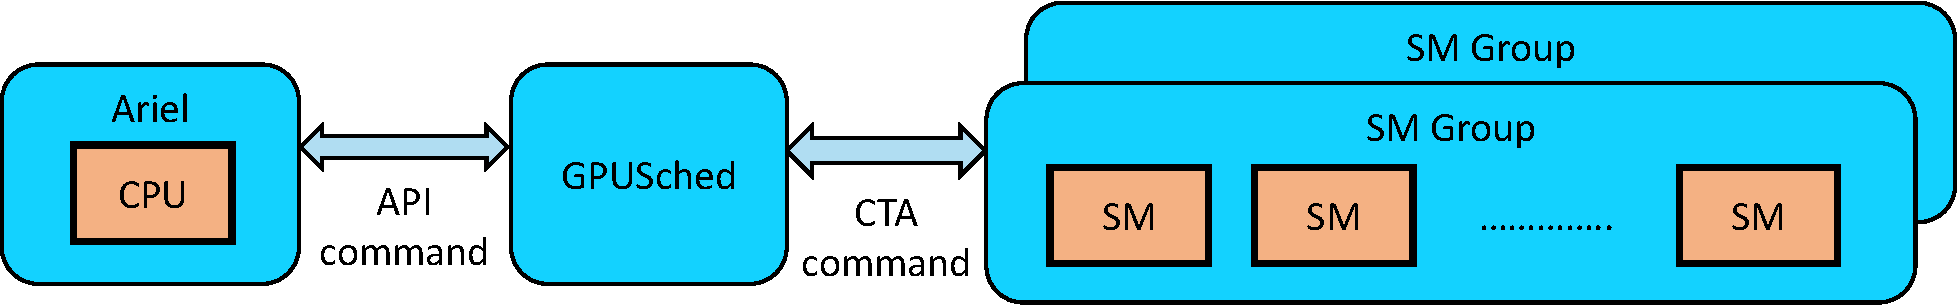
\includegraphics[width=.90\textwidth,keepaspectratio]{figures/2_1-eps-converted-to-crop.pdf}
      \captionsetup{width=.90\textwidth}
      \caption{SST Element architecture for kernel/CTA scheduler and SMs components}
      \label{fig:gpu_sched}
   \end{figure}


As CTAs complete on the SMs, messages are sent back to the GPU scheduler
element, which pushes new work to the SMs from enqueued kernels as needed.
Memory copies from the CPU to GPU address space are handled on a configurable
page-size granularity, similar to how conventional CUDA unified memory handles
the transfer of data from CPU to GPU memories.

   \begin{figure}[!htb]
      \centering
      \setlength{\abovecaptionskip}{6pt plus 1pt minus 1pt}
      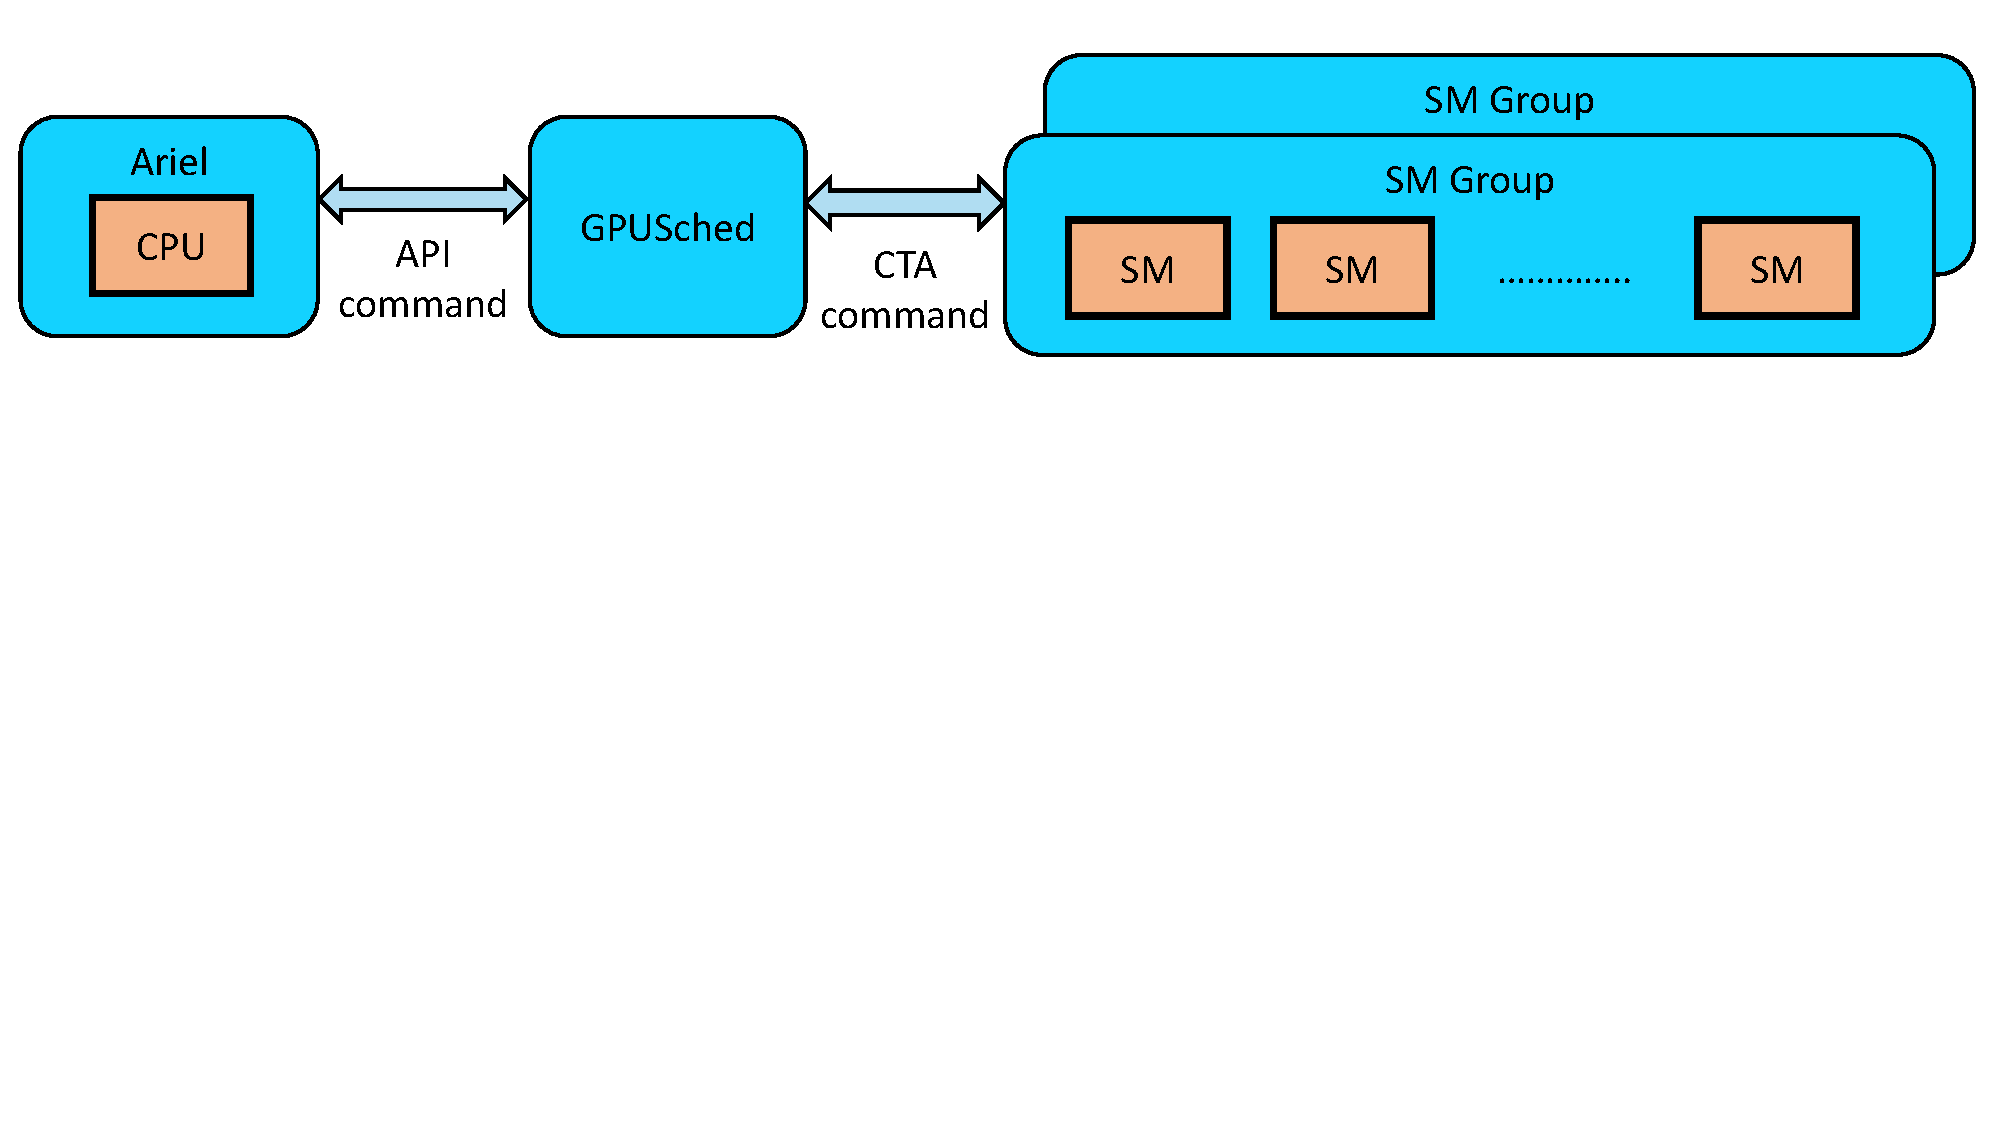
\includegraphics[width=.90\textwidth,keepaspectratio]{figures/scheduler.pdf}
      \captionsetup{width=.75\textwidth}
      \caption{Centralized GPU Scheduler component}
      \label{fig:sched}
   \end{figure}

The centralized GPU scheduler receives kernel launch commands from the CPU, then
issues CTA launch commands to the SMs. The scheduler also receives notifications
from the SMs when the CTAs finish. The reception of kernel launch and CTA
complete notifications are independent, therefore we designed a different
handler for each type of message. Figure~\ref{fig:sched} shows the design of the
centralized kernel and CTA Scheduler. The kernel handler listens to calls from a
CPU component and pushes kernel launch information to the kernel queue when it
receives kernel configure and launch commands. The SM map table contains CTA
slots for each of the SMs, which is reserved when launching a CTA and released when a
message indicating that a CTA has finished is received from the SMs. The
scheduler clock ticks trigger CTA launches to SMs, when space is available and
there is a pending kernel. On every tick, the scheduler issues a CTA launch
command for currently unfinished kernels if any CTA slot is available or tries
to fetch a new kernel launch from kernel queue. The CTA handler also waits for
SMs to reply the CTA finish message, so that CTA slots in the SM map table may
be freed.

To support the GPGPU-Sim functional model, a number of the simulator's overloaded
CUDA Runtime API calls were updated. Several functions that originally assumed
the application and simulator were within the same address space now support them being
decoupled. Initialization functions, such as \texttt{\textunderscore \textunderscore
cudaRegisterFatBinary}, now take paths to the original application to obtain the PTX
assembly of CUDA kernels.


   \begin{figure}[!htb]
      \centering
      \setlength{\abovecaptionskip}{6pt plus 1pt minus 1pt}
      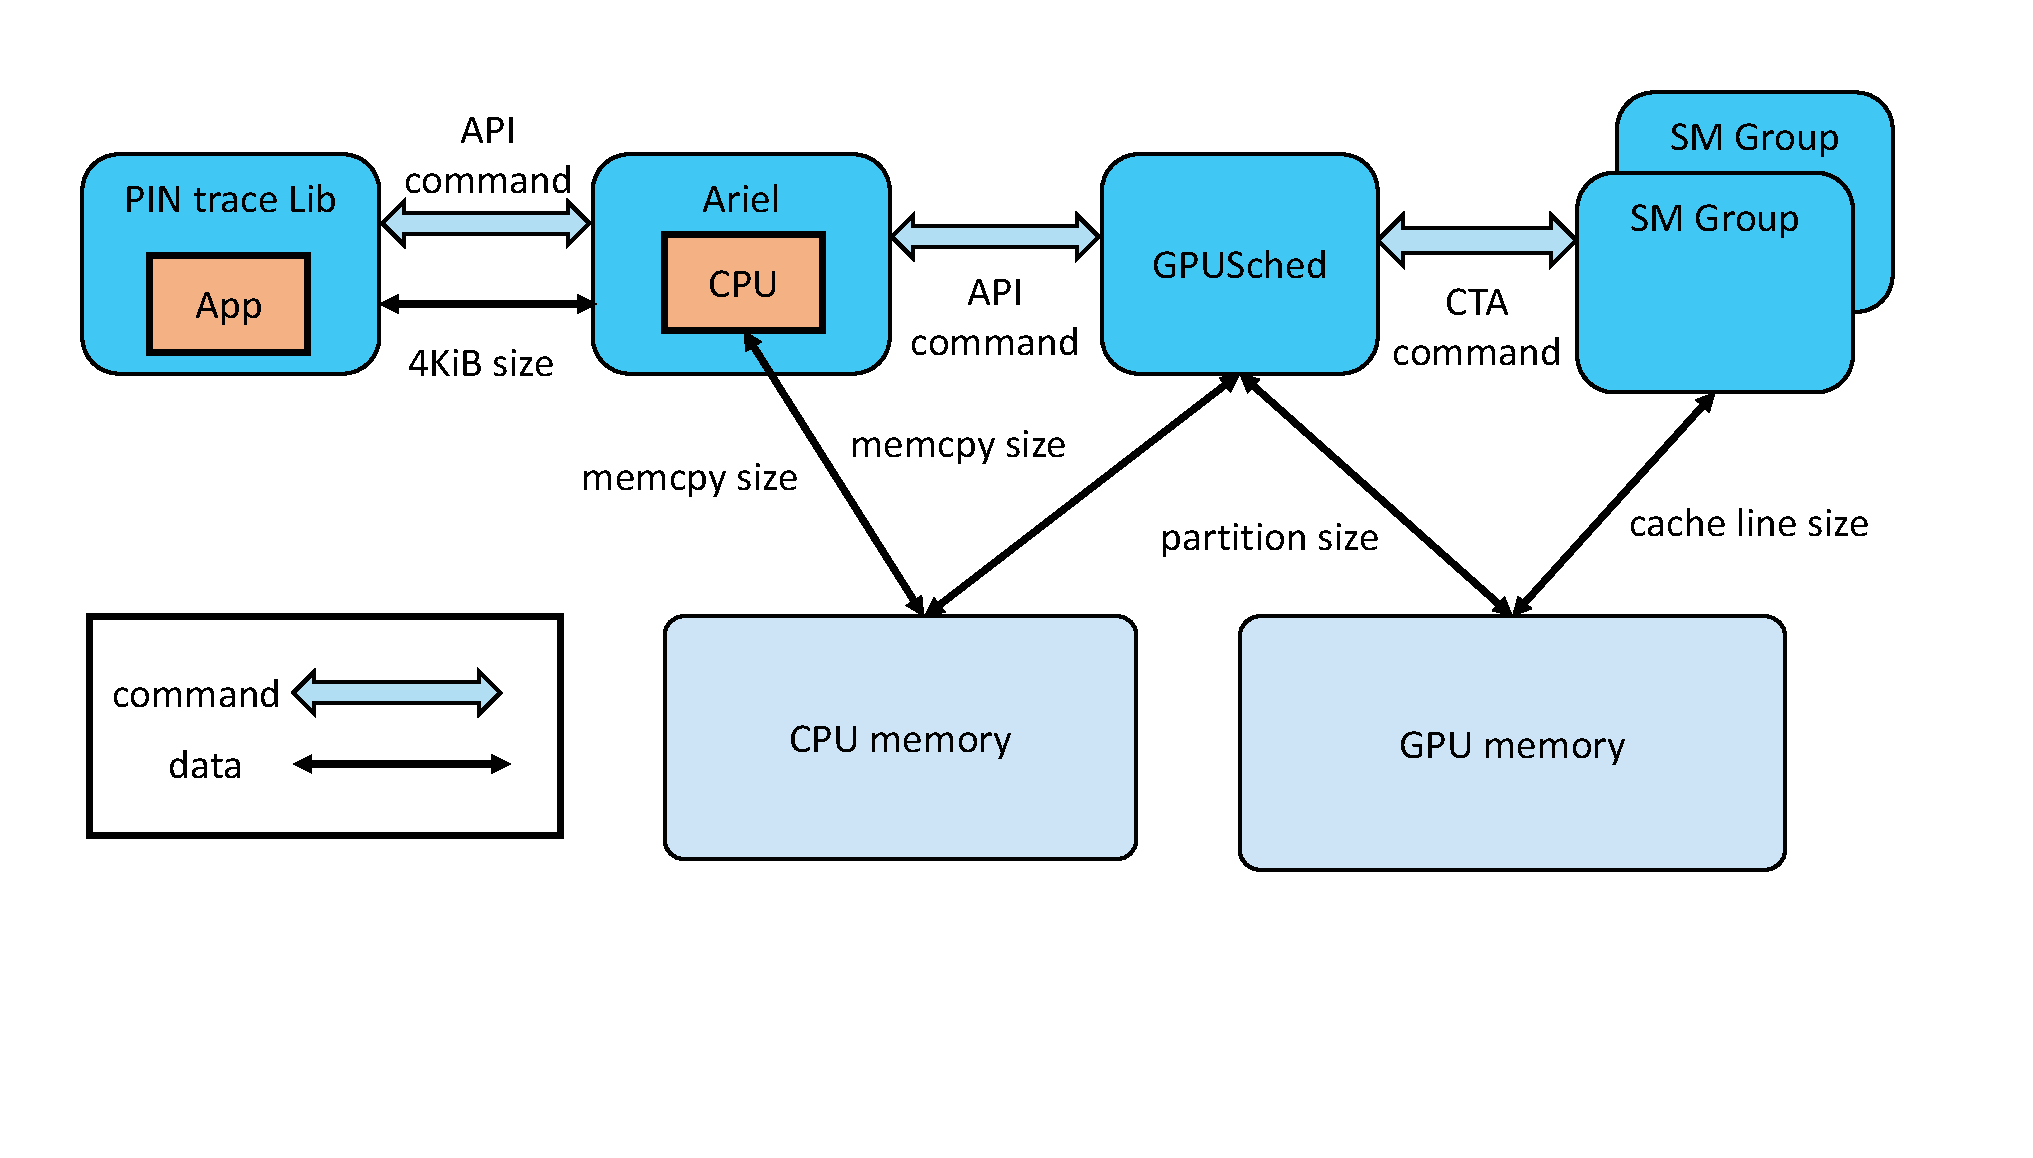
\includegraphics[width=.90\textwidth,keepaspectratio]{figures/transfer_flow.eps}
      \captionsetup{width=.75\textwidth}
      \caption{Data transfer flow for functional simulation}
      \label{fig:gpu_transfer_model}
   \end{figure}

Supporting the functional model of GPGPU-Sim also requires transferring values
from the CPU application to the GPU memory system. This is solved by leveraging
the link between CPU/GPU and memory hierarchy from SST, as shown in
\ref{fig:gpu_transfer_model}. Before actually storing values to memory, appropriate 
CPU memory and GPU memory spaces need to be allocated. As a matter of fact, both CPU memory 
and GPU memory are pre-allocated, and their sizes are set in the configuration file. 
Therefore, the rest of \"allocation\" just needs to avoid collision. A simple way to do this is
keeping a pointer to the current boundry of heap but at the cost of unable to free memory chunks. 
CPU memory allocation is done by Ariel in the CPU simulation -- an option argument is set inside 
configuration file to intercept memory allocation, but other load/store instructions are ignored for 
the time reason. \texttt{malloc} is sent from application to Ariel and the MMU of Ariel takes 
over to settle page allocation; while GPU memory allocation is completed by the 
GPU Scheduler. Unlike the Ariel, there's no MMU inside the GPU so the only thing \texttt{cudaMalloc} 
needs to do is to move the pointer.

Data are transferred from the application to Ariel through
inter-process communication tunnels when \texttt{cudaMalloc} is called. 
Ariel then communicates with the GPU scheduler through
the CPU memory. The GPU scheduler then writes the data to the GPU memory. When an SM
requests a piece of data, the SM accesses the GPU memory for it.
The tunnels utilize 4KiB size as the granularity, while the CPU and the GPU Scheduler
employ larger size non-cacheable requests to access to the CPU memory. When it comes to
GPU memory, some particular attention needs to be paid. The GPU Scheduler communicates with 
the GPU memory in partition size because only one partition can be accessed at a single time. 
The SM transfers data to/from the GPU memory in cache line size because store/load 
instructions manipulate data in cache line granularity (more details in next paragraph). 

To model GPU performance, the memory system of the public GPGPU-Sim is
completely removed. Instead, all accesses to GPU memory are sent though SST
links to the MemHierarchy interface. As Figure \ref{fig:gpu_mem_model} shows, a
multi-level cache hierarchy is simulated with the shared L2 sliced between
different memory partitions, each with its own memory controller. Several
backend timing models have been configured and tested, including SimpleMem,
SimpleDRAM, TimingDRAM, and CramSim \cite{healy2017}; CramSim will be used to
model the HBM stacks in the more detailed performance models. We have created an
initial model for the GPU system similar to that found in an Nvidia Volta. The
configuration for the GPU, CramSim and Network components is shown in Listing
\ref{lst:sst_config}.


\lstdefinelanguage{mooCows}
{
  basicstyle={\small\ttfamily},
  columns=flexible,
  tag=[s]{[]},
  tagstyle=\color{dkgreen}\bfseries,
  usekeywordsintag=true
}[html]

\lstset{frame=tb,
  language=mooCows,
  aboveskip=3mm,
  belowskip=3mm,
  showstringspaces=false,
  columns=flexible,
  basicstyle={\small\ttfamily},
  numbers=none,
  numberstyle=\tiny\color{gray},
  breaklines=true,
  breakatwhitespace=true,
  tabsize=3
}

\lstinputlisting[caption=Sample SST-GPGPU Configuration, label=lst:sst_config]{figures/config}


To evaluate the performance correlation of our GPU-SST model, versus both real
hardware and the existing GPGPU-Sim memory system implementation an execution
time correlation is done on the vectorAdd benchmark from the CUDA SDK. Figure
\ref{fig:titanv_result} shows the results of this timing analysis. The most
accurate GPGPU-Sim timing model is reasonably accurate (within 25\% of the
hardware results), however GPU-SST is much closer to real hardware, showing
just and 8\% deviation from a silicon Nvidia Titan V card.


   \begin{figure}[!htb]
      \centering
      \setlength{\abovecaptionskip}{6pt plus 1pt minus 1pt}
      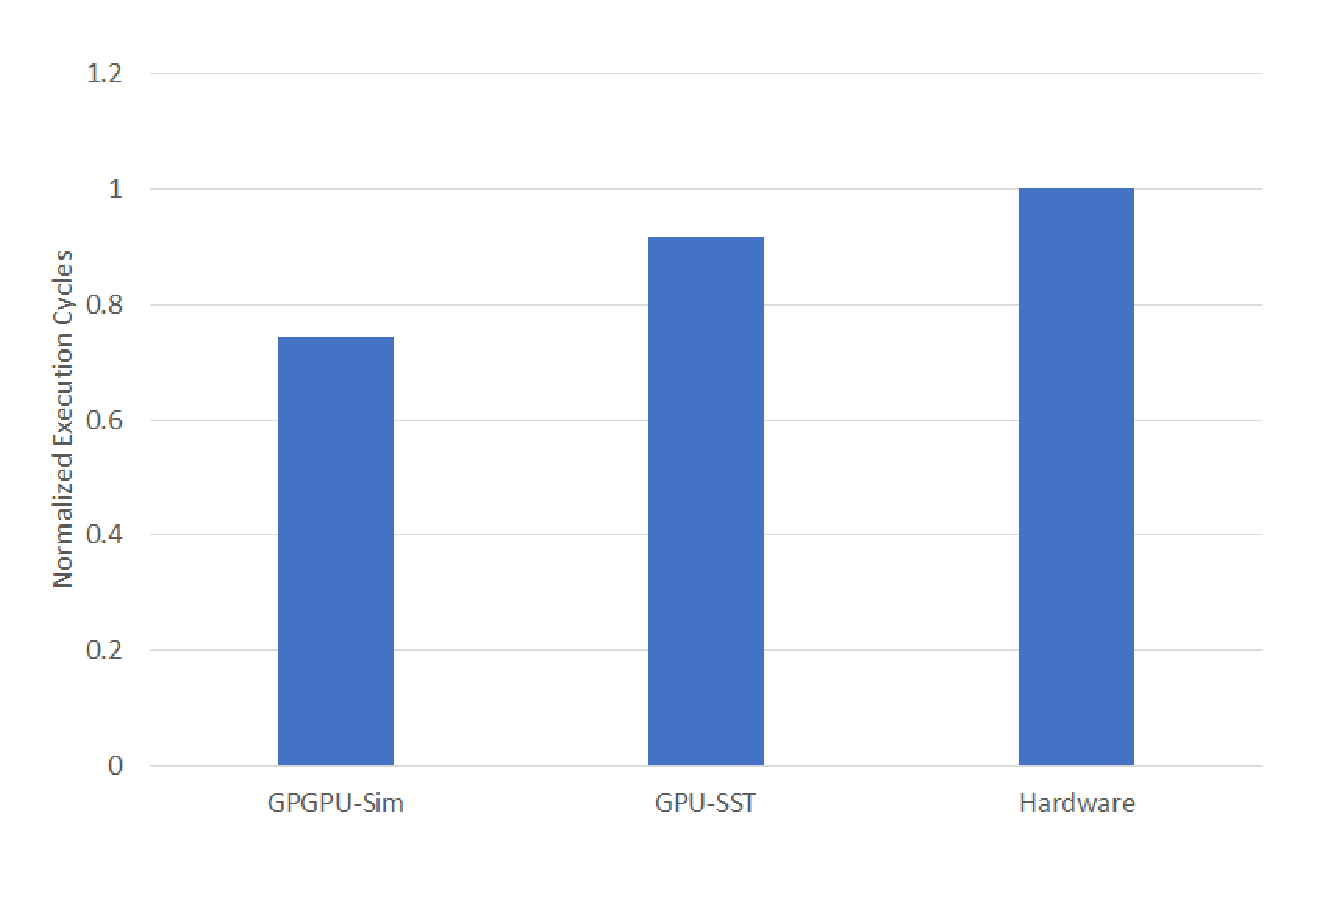
\includegraphics[width=.50\textwidth,keepaspectratio]{figures/4_1.eps}
      \captionsetup{width=.90\textwidth}
      \caption{Normalized execution time for 160k element vector addition kernel -- \\
               SST-GPU is within 8\% of the silicon of the Titan V}
      \label{fig:titanv_result}
   \end{figure}

This report has detailed the first phase of the SST-GPU project, where the
execution-driven functional and performance model of a GPU had been integrated
SST. Initial results demonstrate significant coverage of applications. The next phase of the project will
focus on further disaggregating the GPU to enable truly scaled GPU performance
in a multi-process MPI simulation.

We would like to thank Gwen Voskuilen for her help with MemHierarchy
and recommendations on debugging problems with the NIC and
interconnect. We would also like to thank Arun Rodrigues and 
Scott Hemmert for their support and help in defining the scope of the project.




\bibliographystyle{IEEEtranS}
\bibliography{sst-gpgpu_perf_SAND/sst_gpgpu_bib}

\end{document}
